\section{Un pò di storia}
%\paragraph{}
A partire dal 1920 si diffondono i primi articoli riguardanti le interferenze radio, dando il via alla ricerca
sui problemi di compatibilità elettromagnetica.
Dieci anni dopo, con lo sviluppo delle industrie che utilizzavano energia elettrica si sono evidenziati i fenomeni
di disturbo e interferenza dovuti alle linee elettriche ferroviarie e all'utilizzo dei motori elettrici.
Durante la II Guerra Mondiale l'utilizzo di comunicazioni radio e sistemi radar fu cruciale per la riuscita
delle missioni, iniziò una vera e propria guerra tecnologica e ci si rese conto della necessità di regolamentare
le trasmissioni sulle varie frequenze.

Tra gli anni '50 e '70 si diffusero i transistor e l'elaborazione digitale dei dati, i circuiti divenivano
sempre più piccoli e commutavano a frequenze sempre più elevate. Questi segnali ad alte frequenze generavano numerosi
disturbi a banda larga in spazi molto ravvicinati fra i vari componenti.

\paragraph{Timeline essenziale} della compatibilità elettromagnetica:

\begin{itemize}
 \item \textbf{1923}: Primi rapporti tecnici sulle interferenze radio
 \item \textbf{1933}: Prime riunioni internazionali per la regolamentazione delle radio interferenze, IEC-UIR
 \item \textbf{1934}: Costituzione del CISPR, con prima riunione a Giugno
 \item \textbf{1979}: Documento da parte della FCC per la limitazione delle emissioni EM dei dispositivi digitali
\end{itemize}


In \textbf{Europa}: 
\begin{itemize}
 \item \textbf{1989}: Direttiva 89/336 in cui si obbligavano i produttori ad occuparsi della 
 Compatibilità Elettromagnetica, modificata da direttive successive nel 92, 93 ed entrò definitivamente in vigore
 nel Gennaio del 1996.
 \item \textbf{1996}: Recepimento in \textbf{Italia} con Decreto Legislativo n° 615.
 \item \textbf{1997-1998}: Pubblicazione delle \textit{guide di applicazione} UE e CEI per interpretare la Direttiva
 Europea.
 \item \textbf{CT 210}: Viene costituito il comitato tecnico 210 nel CENELEC e nel CEI riguardo la compatibilità
 elettromagnetica.
 \item \textbf{108/04/CE}: Direttiva a valle del progetto \textit{SLIM} al fine di semplificare la legislazione.
\end{itemize}

\paragraph{La direttiva Europea}
Documento mediante il quale l'Unione regola il commercio nel Mercato Interno, il produttore di un'apparecchiatura
deve fornire una \textit{``Dichiarazione di Conformità''} contenuta nel \textit{``Technical Construction
File''} che descriva il prodotto e ne illustri la conformità al fine di ottenere il marchio \textbf{CE}.

Nel \textit{1997} l'iniziativa nota come \textbf{SLIM} (Simplified Legislation for the Internal Market)
evidenziò la necessità di semplificare le normative mantenendo comunque un elevato livello di sicurezza.

Nel ``Nuovo Approccio'' la direttiva indica solo quali sono gli obiettivi da raggiungere ma non come farlo
per non limitare il progresso tecnologico. Le specifiche tecniche da rispettare vengono poi illustrate
nelle Norme Armonizzate, emanate da organizzazioni come il CENELEC, risulta in questo modo molto più semplice
aggiornare una Norma Armonizzata per modificare, ad esempio, i range di frequenza piuttosto che agire sull'intera 
Direttiva Europea, che richiederebbe un lavoro politico e burocratico molto più intenso.

\section{Gli apparati coinvolti}
L'articolo 2.1 della direttiva 108/04/CE distingue:
\begin{itemize}
 \item \textbf{Apparecchiatura}: Ogni apparecchio o impianto fisso
 \item \textbf{Apparecchio}: Dispositivo finito o combinazione di dispositivi finiti, commercializzati come unità 
 funzionali e destinati all'utente finale
 \item \textbf{Impianto fisso}: Combinazione particolare di apparecchi assemblati ed installati per essere
 utilizzati in un solo luogo
\end{itemize}

I dispositivi interessati coprono una grande varietà di settori, a partire dagli elettrodomestici agli apparecchi
per l'informazione, gli apparati per l'illuminazione, le macchine industriali fino alle apparecchiature 
elettromedicali.

La verifica della conformità \textbf{EMC} viene eseguita seguendo le Norme Armonizzate e il risultato delle prove viene
riportato nel \textit{Technical Construction File}, i prodotti che rispettano gli standard di prodotto, (o in assenza
di questi gli standard generici) vengono ritenuti conformi alla direttiva EMC e per questo viene prodotta la
dichiarazione di conformità e rilasciato il marchio CE.
Non è richiesta la marchiatura CE per le installazioni fisse dato che non devono essere commercializzate
tra i paesi membri ma devono solo garantire il corretto funzionamento nel punto in cui vengono installate.
La dichiarazione di conformità può prevedere una autocertificazione o l'intervento di un'autorità esterna per la
revisione della documentazione.

La differenza fra l'autocertificazione o l'intervento dell'autorità esterna è determinata dalla criticità del settore
in cui l'apparecchiatura deve funzionare (es. ambienti medicali, militari ecc...).

La verifica della conformità alla Direttiva EMC non solo consente il libero scambio di prodotti nel mercato europeo
ma permette comunque di realizzare un prodotto di livello superiore, con una maggiore robustezza ai disturbi e una
maggiore compatibilità anche in ambienti elettricamente ``affollati''.

\section{Gli organismi coinvolti}
Nel controllo del rispetto della Direttiva Europea sono coinvolti numerosi organismi e autorità:
Le \textbf{Autorità Competenti} sono enti riconosciuti dai singoli stati ai quali è stato affidato il compito
di vigilare sul mercato e controllare i prodotti che vi transitano, ad esempio le \underline{Camere di commercio}

Gli \textbf{Organismi Competenti} dimostrano di avere le competenze tecniche per verificare le caratteristiche di un 
apparato. Non eseguono le misurazioni sugli apparecchi ma sono in grado di analizzare e valutare
i risultati delle stesse.

Gli \textbf{Organismi Notificati} a cui è demandata, da parte delle Autorità Competenti, la verifica delle
caratteristiche di conformità alla direttiva EMC mediante le misure. Le certificazioni rilasciate dagli organismi
notificati sono già ritenute valide dalla Comunità Europea.

Un organismo competente o notificato deve avere disponibilità di attrezzatura specifica e personale specializzato,
non deve avere alcun conflitto di interessi con l'azienda che richiede la certificazione; deve essere sottoposto a 
verifica periodica. Le sue dichiarazioni hanno validità legale e deve essere assicurato sulla responsabilità civile
delle proprie dichiarazioni.

\begin{figure}[h]
 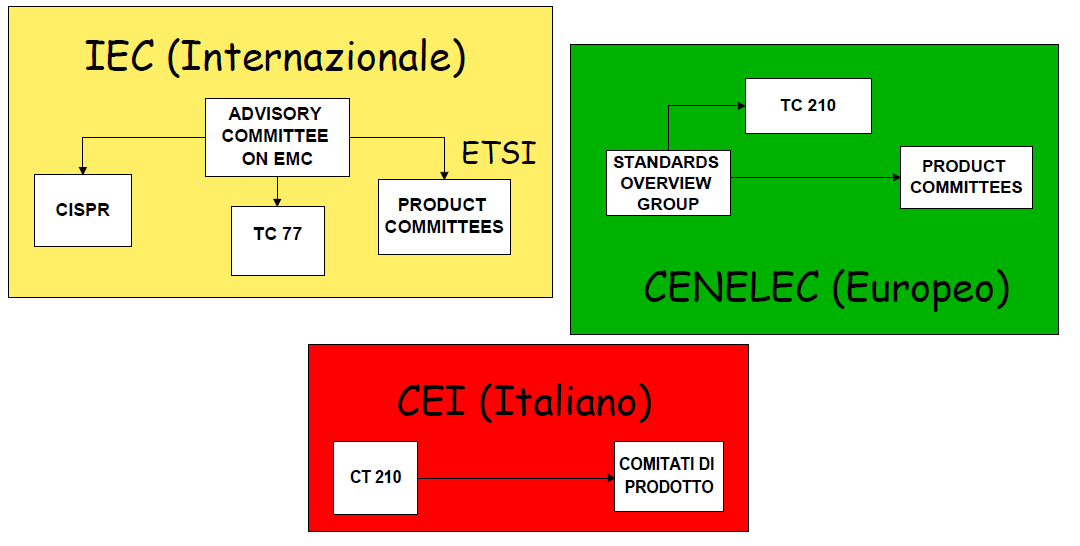
\includegraphics[width=0.7\linewidth]{enti.png}
 \centering
 \caption{Organismi di Normazione}
 \label{fig:enti}
\end{figure}

Tutti i paesi interessati partecipano all'IEC, le Norme attuate in Europa vengono invece rilasciate dal CENELEC mentre
il CEI in Italia collabora con i comitati di prodotto per redigere le norme.
L`IEC non è gerarchicamente superiore al CENELEC, nonostante sia un comitato internazionale non ha potere
sull'Europa, deve essere il CENELEC a recepire ed armonizzare una eventuale norma rilasciata dall'IEC.
L'Italia può avere una propria normazione tecnica ma se ci dovessero essere norme in contrasto con le normative 
Europee, queste dovranno essere aggiornate ed adeguate alla normazione più generale (europea). In teoria il singolo
Stato potrebbe avere normative più stringenti, ma queste potrebbero portare a ricorsi da parte dei produttori
che non potrebbero vendere i loro prodotti nei determinati stati membri, nonostante siano ``a norma''
secondo la Comunità Europea.




